\documentclass[11pt,a4paper]{article}

\usepackage{pifont}
\usepackage{amsmath}
\usepackage{amssymb}
\usepackage{graphicx}
\usepackage{array}
\usepackage{fancyheadings}
\usepackage{here}
\usepackage{pslatex}
\usepackage{eepic,epic}
\usepackage[english]{babel}
\usepackage[dvips,pageanchor=true,hyperindex=true,pagebackref=true,pdfhighlight=/O,pdfauthor={Yves Renard}]{hyperref}%pour le pdf

\usepackage{fancyheadings}
\usepackage{amsmath}
\usepackage{amssymb}
\usepackage{psfig}
\usepackage{here}
\usepackage{array}
\usepackage{alltt}
\usepackage{graphicx}
\usepackage{eepic,epic}
\usepackage[latin1]{inputenc}
\usepackage[T1]{fontenc}
% \usepackage[french]{babel}
% \usepackage[dvips]{epsfig}

%\oddsidemargin -0.2cm
%\evensidemargin -0.2cm
%\topmargin -1cm
%\textheight 22.5cm
%\textwidth 16.2cm
%\headheight 1.0cm

\newfont{\eufmtwelve}   {eufm10 scaled \magstep1}
\newfont{\eufmten}      {eufm10 }
\newfont{\eufmnine}     {eufm9 }
\newfont{\eufmeight}    {eufm8 }
\newfont{\eufmseven}    {eufm7 }
\newfont{\eufmsix}      {eufm6 }
\newfont{\eufmfive}     {eufm5 }
\newfont{\eusmtwelve}   {eusm10 scaled \magstep1}
\newfont{\eusmten}      {eusm10}
\newfont{\eusmnine}     {eusm9 }
\newfont{\eusmeight}    {eusm8 }
\newfont{\eusmseven}    {eusm7 }
\newfont{\eusmsix}      {eusm6 }
\newfont{\eusmfive}     {eusm5 }
\newfont{\msbmtwelve}   {msbm10 scaled \magstep1}
\newfont{\msbmeight}    {msbm8}

\newcommand{\udl}{\underline}
\newcommand{\udll}[1]{{\udl{\udl{#1}}}}
\newcommand{\udlll}[1]{{\udl{\udl{\udl{#1}}}}}
\newcommand{\mat}[1]{{\mbox{\msbmtwelve {#1}}}}
\newcommand{\Reel}{{\mbox{\msbmtwelve R}}}      % L'ensemble des reels.
\newcommand{\reel}{{\mbox{\msbmeight R}}}       % L'ensemble des reels.
%\newcommand{\Reel}{{\rm I\hspace{-0.15em}R}}
\newcommand{\Complex}{\mbox{\msbmtwelve C}}     % L'ensemble des complexes.
\newcommand{\Naturel}{\mbox{\msbmtwelve N}}  % L'ensemble des entiers naturels.
\newcommand{\naturel}{\mbox{\msbmeight N}}   % L'ensemble des entiers naturels.

%\newcommand{\Naturel}{{\rm I\hspace{-0.15em}N}}% L'ensemble des entiers naturels.
\renewcommand{\emptyset}{\mbox{$\circ$\hspace{-.50em}/}}  % ensemble vide.
\newcommand{\Cont}{{\cal C}}            % L'ensemble des fonctions continues
\newcommand{\Cinf}{{\cal C}^{\infty}}   % L'ensemble des fonction C-infinies
\renewcommand{\vec}[1]{\overrightarrow{\!\!#1}}
\newcommand{\subsetcont}{{\subset\hspace{-.6em}_{\scriptscriptstyle >} }}
\newcommand{\Frac}[2]{{\ds \frac{\ds #1}{\ds #2}}}
\newcommand{\interior}[1]{{\stackrel{\circ}{#1}}}
\newcommand{\cqfd}{{$\mbox{}$\hfill\rule{2.5mm}{2.5mm}}}
\newcommand{\vectwo}[2]{{\left(\hspace{-.5em}\begin{array}{c} {#1} \\ {#2}
     \end{array}\hspace{-.5em}\right)}}
\newcommand{\vecthree}[3]{{\left(\hspace{-.5em}\begin{array}{c} {#1}
     \\ {#2} \\ {#3} \end{array}\hspace{-.5em}\right)}}
\newcommand{\vecfour}[4]{{\left(\hspace{-.5em}\begin{array}{c} {#1}
     \\ {#2} \\ {#3} \\ {#4} \end{array}\hspace{-.5em}\right)}}
\newcommand{\vecfive}[5]{{\left(\hspace{-.5em}\begin{array}{c} {#1}
     \\ {#2} \\ {#3} \\ {#4} \\ {#5} \end{array}\hspace{-.5em}\right)}}
\newcommand{\vecseven}[7]{{\left(\hspace{-.5em}\begin{array}{c} {#1}
     \\ {#2} \\ {#3} \\ {#4} \\ {#5} \\ {#6} \\ {#7} \end{array}\hspace{-.5em}\right)}}
\def\infess{\mathop{\iflanguage{english}{\mbox{ess$\,$inf}}{\mbox{inf$\,$ess}}}}
\def\supess{\mathop{\iflanguage{english}{\mbox{ess$\,$sup}}{\mbox{sup$\,$ess}}}}
\def\essinf{\mathop{\iflanguage{english}{\mbox{ess$\,$inf}}{\mbox{inf$\,$ess}}}}
\def\esssup{\mathop{\iflanguage{english}{\mbox{ess$\,$sup}}{\mbox{sup$\,$ess}}}}
\def\aplim{\mathop{\mbox{ap$\,$lim}}}
\def\aplimsup{\mathop{\mbox{ap$\,$lim$\,$sup}}}
\def\apliminf{\mathop{\mbox{ap$\,$lim$\,$inf}}}
\def\convto{\mathop{\hbox{\rightarrowfill}}} % converge vers.
\newcommand{\rightgap}{{]\hspace{-0.12em}]}}
\newcommand{\leftgap}{{[\hspace{-0.12em}[}}
\newcommand{\gapof}[1]{{\leftgap {#1} \rightgap}}
\newcommand{\restrictiona}[1]
{{ \begin{picture}(13,10) \put(-1,-4){$\mid_{#1}$} \end{picture}
}} % Le signe "Restriction sur #1"

\def\Indic{\mbox{1\hspace{-0.20em}I}}   % Fonction l'indicatrice

% \def\bar3{|\hspace{-1pt}\|} % 3bar verticaux pour les normes matricielles.
\def\cvweak{\mathop{-\hspace{-0.3em}-\hspace{-0.6em}\rightharpoonup}} % fleche cv faible
\def\cvweakstar{\cvweak^*} % fleche cv faible etoile
\def\longmapsto
{ \begin{picture}(0,10)
  \put(0,0){$\scriptstyle{\vdash}$} \end{picture} \mbox{$\longrightarrow$}
} 

\def\build#1_#2^#3{\mathrel{
 \mathop{\kern 0pt#1}\limits_{#2}^{#3}}} % Ecrire en dessous et dessus un symbole.

\def\Dist{\mbox{\eusmtwelve D}} %signe de distribution
\def\dist{\mbox{\eusmten D}} %signe de distribution


%definition de commandes utilises
\newcommand{\ds}{\displaystyle}
\newcommand{\rc}{{\par}}
\newcommand{\rcc}{{\par\medskip}}
\newcommand{\rccc}{{\par\bigskip}}


%definition des environnements theoreme, lemme, ...
\usepackage{boxedminipage}
% \newenvironment{largebox}
%   { \rc\noindent \begin{boxedminipage}[t]{\textwidth} }
%   { \end{boxedminipage}  \rccc\noindent }
\newenvironment{largebox}
  { \rc\noindent \begin{boxedminipage}[t]{\linewidth} }
  { \end{boxedminipage}  \rccc\noindent }


\newtheorem{ltheoreme}{Th\'eor\`eme}
\newenvironment{theoreme}
  { \begin{largebox} \begin{ltheoreme} }
  { \end{ltheoreme} \end{largebox} }
\newtheorem{lproposition}{Proposition}
\newenvironment{proposition}
  { \begin{largebox} \begin{lproposition} }
  { \end{lproposition} \end{largebox} }
\newtheorem{llemme}{Lemme}
\newenvironment{lemme}
  { \begin{largebox} \begin{llemme} }
  { \end{llemme} \end{largebox} }
\newtheorem{ldefinition}{D\'efinition}
\newenvironment{definition}
  { \begin{largebox} \begin{ldefinition} }
  { \end{ldefinition} \end{largebox} }
\newtheorem{lhypothese}{Hypoth\`ese}
\newenvironment{hypothese}
  { \begin{largebox} \begin{lhypothese} }
  { \end{lhypothese} \end{largebox} }
\newtheorem{lcorollaire}{Corollaire}
\newenvironment{corollaire}
  { \begin{largebox} \begin{lcorollaire} }
  { \end{lcorollaire} \end{largebox} }
\newenvironment{remarque}
  { \begin{largebox} {\bf \udl{Remarque} : }}
  { \end{largebox} }

\newcounter{numberofprobl}
\setcounter{numberofprobl}{1}

\newlength{\compteurtpourprobla}
\newlength{\compteurtpourproblb}
\newenvironment{caseeqnarray}[1]
  {
   $${#1}
   \settowidth{\compteurtpourprobla}{${#1}\left\{\right.$}
   \setlength{\compteurtpourproblb}{\textwidth}
   \addtolength{\compteurtpourproblb}{-1\compteurtpourprobla}
   \settowidth{\compteurtpourprobla}{$\;$}
   \addtolength{\compteurtpourproblb}{-1\compteurtpourprobla}
   \left\{ \begin{minipage}[l]{\compteurtpourproblb}
   \vspace{-1em} \begin{eqnarray}
  }
  { \end{eqnarray} \end{minipage} \right. $$}


\newtheorem{hypothesis}{Hypothesis}
\newtheorem{prop}{Proposition}
\newtheorem{defi}{Definition}
%\newtheorem{theorem}{Theorem}
%\newtheorem{lemma}{Lemma}


% pour plus tard ...
% \DeclareGraphicsRule{ps.Z}{eps}{ps.bb}{`zcat #1}
% \DeclareGraphicsRule{eps.Z}{eps}{eps.bb}{`zcat #1}
% \DeclareGraphicsRule{ps.gz}{eps}{ps.bb}{`gunzip #1}
% \DeclareGraphicsRule{eps.gz}{eps}{eps.bb}{`gunzip #1}


\oddsidemargin -0.4cm
\evensidemargin -0.4cm
\topmargin -1cm
\textheight 22.5cm
\textwidth 16.6cm
\headheight 1.0cm

% principal notations



\begin{document}

\begin{center}
  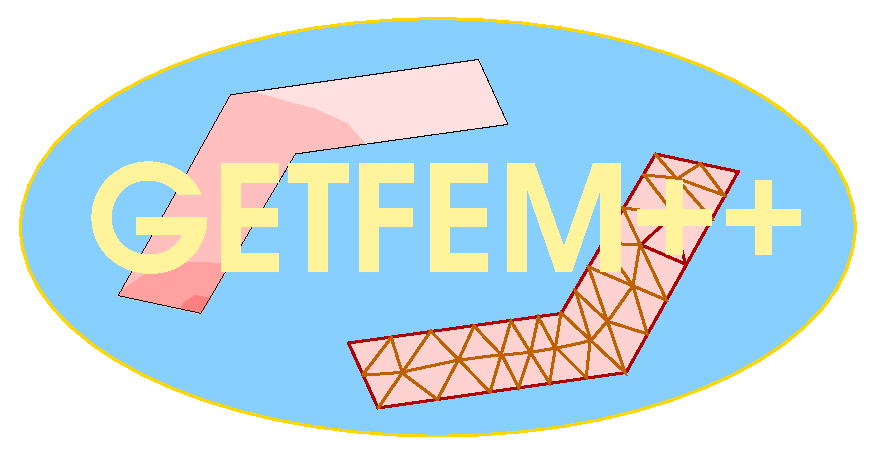
\includegraphics[width=10cm,angle=0]{getfem_logo.eps}\\[0.2cm]
  a Generic Finite Element library in C++ \\[0.5cm]
  {\LARGE Documentation, part \Huge 1} \\[0.5cm]
  \fbox{\Huge \sc Elementary Computations} \\[0.5cm]
  { \large Yves \sc Renard\footnote{ \it MIP, INSAT, Complexe scientifique de Rangueil, 31077 Toulouse, France, Yves.Renard@gmm.insa-tlse.fr } } \\[1.0cm]
      \today \\[1.0cm]
\end{center}

% \begin{abstract}
% Basic description of the structure of the finite element kernel of {\sc Getfem++}.
% \end{abstract}


%%%%%%%%%%%%%%%%%%%%%%%%%%%%%%%%%%%%%%%%%%%%%%%%%%%%%%%%%%%%%%%%%%%%%%%%%
%          INTRODUCTION                                                 %
%%%%%%%%%%%%%%%%%%%%%%%%%%%%%%%%%%%%%%%%%%%%%%%%%%%%%%%%%%%%%%%%%%%%%%%%%

\section*{Introduction}
The main goal of {\sc Getfem++} is to use C++ language facilities to build an advanced finite element library easy to use, as complete as possible and efficient. Here is presented the finite element kernel of this project. A particular attention has been paid to reduce the computation time. The finite element kernel has been built in order to take into account from the simplest methods ($P_K$ methods on simplices with a linear geometric transformation) to the more elaborated methods (Hermite elements, vectorial elements, non-polynomials elements ...). Once a finite element method is described on the reference element, arbitrary elementary  matrices can be computed, even elementary matrices for mixed methods. The code is generic in the sense that there is no limitation in dimension and degree and existing assembling procedures are completely independent of the dimension and the finite element methods used.\\[2.4cm]
Copyright (C) 2000-2020 Yves Renard, Julien Pommier.\\
The program GetFEM is free software; you can redistribute it and/or modify
it under the terms of the GNU Lesser General Public License as published by
the Free Software Foundation; either version 3 of the License, or
(at your option) any later version along with the GCC Runtime Library
Exception either version 3.1 or (at your option) any later version.
This program is distributed in the hope that it will be useful,
but WITHOUT ANY WARRANTY; without even the implied warranty of
MERCHANTABILITY or FITNESS FOR A PARTICULAR PURPOSE.  See the
GNU Lesser General Public License for more details.
You should have received a copy of the GNU  Lesser General Public License
along with this program; if not, write to the Free Software Foundation,
Inc., 51 Franklin Street, Fifth Floor, Boston, MA  02110-1301  USA

\newpage
\tableofcontents
\newpage


\section{Convex structures}
Finite element methods are defined on small convex domains called elements. The simplest element on which a finite element method can be defined is a segment (simplex of dimension 1), other possibilities are triangles, tetrahedrons (simplices of dimension 2 and 3), prisms, parallelepiped ...
As we want to define a generic library, we need an object which describes the structure of an element (for us, a convex). This description is made by an object defined in the file {\tt bgeot\_convex\_structure.h } which is\\[0.5cm]
{\tt bgeot::convex\_structure }\\[0.5cm]
It describes the information needed such as the number of vertices, of faces, the dimension, etc ... It describes only the structure of the convex not the coordinates of the vertices.
This structure is not to be manipulated by itself, because it is not necessary that more than one structure of this type describe the same convex. What will be manipulated is a pointer on such a  descriptor which has to be declared with the type\\[0.5cm]
{ \tt bgeot::pconvex\_structure } \\ \\

To have a description of a convex, one calls the following functions

\begin{center} \begin{tabular}{|m{0.55\linewidth}|m{0.4\linewidth}|} \hline
  {\tt bgeot::pconvex\_structure bgeot::simplex\_structure(dim\_type d)} & description of a simplex of dimension {\tt d}. \\ \hline
  {\tt bgeot::pconvex\_structure bgeot::parallelepiped\_structure(dim\_type\;d)} &  description of a parallelepiped of dimension {\tt d}. \\ \hline
  {\tt bgeot::pconvex\_structure bgeot::convex\_product\_structure( bgeot::pconvex\_structure p1, bgeot::pconvex\_structure p2) } & description of the direct product of {\tt p1} and {\tt p2}.\\ \hline
  {\tt bgeot::pconvex\_structure bgeot::prism\_structure(dim\_type d)}  & description of a prism of dimension {\tt d}\\ \hline
\end{tabular} \end{center}

For instance if one needs the description of a square, one can call either

{\tt p = bgeot::parallelepiped\_structure(2); }

or

{\tt p = bgeot::convex\_product\_structure(bgeot::simplex\_structure(1),\\        \mbox{} \hspace{18.5em} bgeot::simplex\_structure(1)); }

which is equivalent.

It is then possible to extract some information such as {\tt p->nb\_faces()} for the number of faces, {\tt p->dim()} for the dimension of the convex, {\tt p->nb\_points()} for the number of vertices. Other information is the number of vertices of each face, the description of a face and the eventual reference to a more basic description (used for the description of geometric transformations).

\begin{figure}[htb]
  \begin{center}
    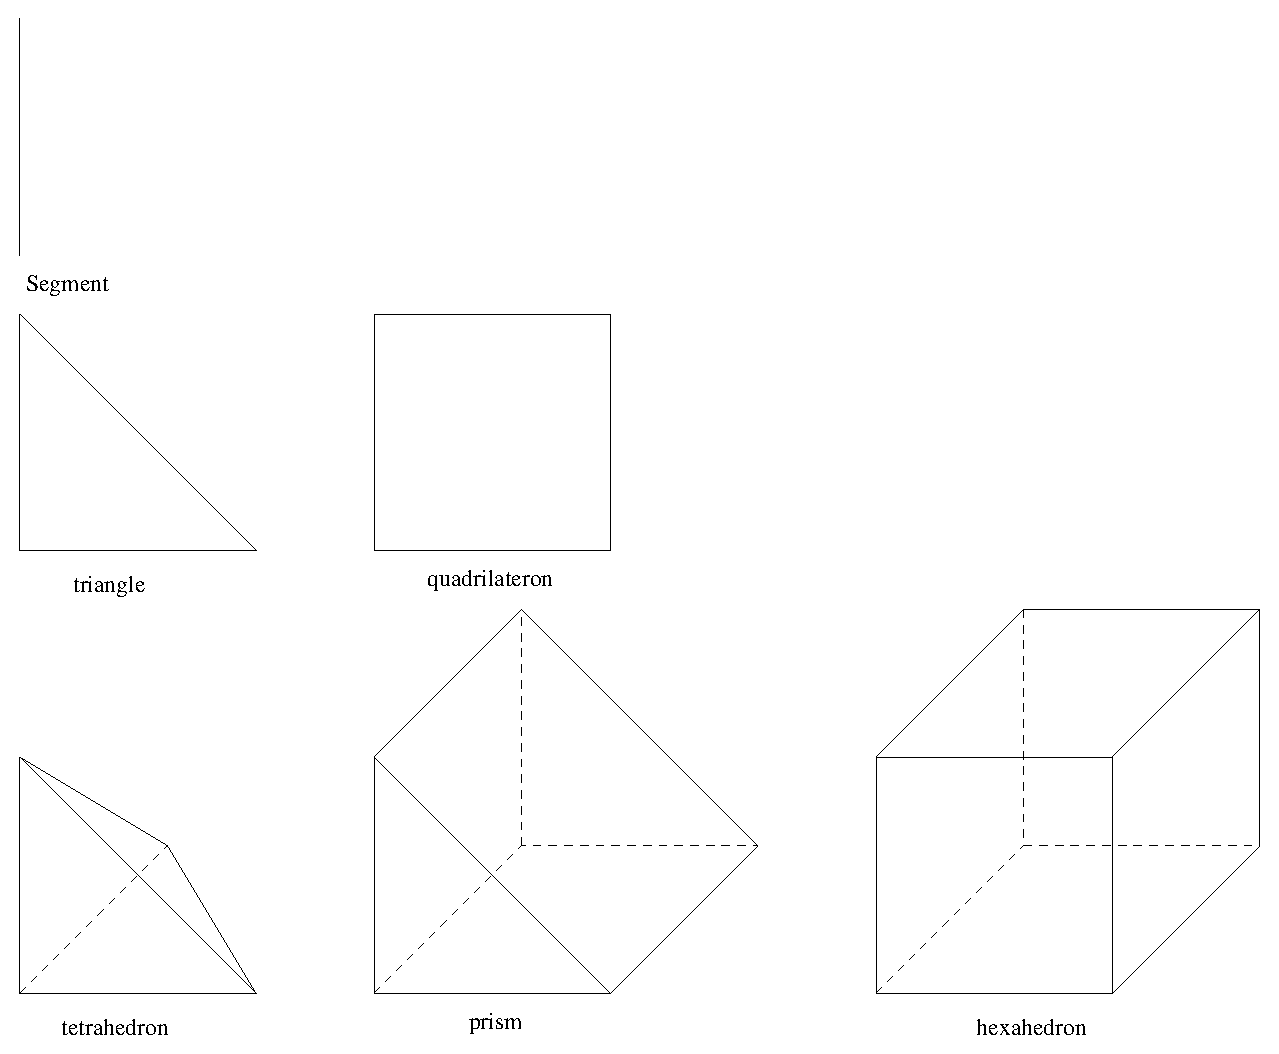
\includegraphics[width=10cm,angle=0]{getfemelem_elem.eps}
  \end{center}
  \caption{ \it usual elements. Elements in higher dimension can also be built }
  \label{fig:elem}
\end{figure}

\rcc

\section{Convexes of reference}

A convex of reference is a particular real element, i.e. a structure of convex with a list of the vertices. It describes the particular element from which a finite element method is defined. In the file {\tt bgeot\_convex\_ref.h} the object\\[0.5cm]
{\tt bgeot::convex\_of\_reference }\\[0.5cm]
makes this description. As it is for the object {\tt bgeot::convex\_structure}, the library keeps only one  description for each type of convex. So what will be manipulated is the type of pointer\\[0.5cm]
{\tt bgeot::pconvex\_ref }\\[0.5cm]
The following functions build the descriptions:

\begin{center} \begin{tabular}{|m{0.55\linewidth}|m{0.4\linewidth}|} \hline
{\tt bgeot::pconvex\_ref $\;$ bgeot::simplex\_of\_reference(dim\_type d)} & description of the simplex of reference of dimension {\tt d} \\ \hline
  
  {\tt bgeot::pconvex\_ref $\;$ bgeot::simplex\_of\_reference(dim\_type d, short\_type k)} & description of the simplex of reference of dimension {\tt d} with degree {\tt k} Lagrange grid. \\ \hline

  {\tt bgeot::pconvex\_ref $\;$ bgeot::convex\_ref\_product(pconvex\_ref a, pconvex\_ref b)} & description of the direct product of two convexes of reference.\\ \hline
  
  {\tt bgeot::pconvex\_ref $\;$ bgeot::parallelepiped\_of\_reference(dim\_type\;d)} & description of the parallelepiped of reference of dimension {\tt d}  \\ \hline
\end{tabular} \end{center}

The vertices correspond to the classical vertices for such reference element. For instance the vertices for the triangle are $(0, 0), (1, 0)$ and $(0, 1)$. It corresponds to the configuration shown in Figure \ref{fig:elem}

If {\tt p} is of type {\tt bgeot::pconvex\_ref } then {\tt p->structure()} is the corresponding convex structure. Thus for example {\tt p->structure()->nb\_points()} gives the number of vertices. The function {\tt p->points()} give the array of vertices, for example {\tt p->points()[0]} is the first vertex. The function {\tt p->is\_in(const base\_node \&pt)} return a real which is negative if the point {\tt pt} is in the element. The function {\tt p->is\_in\_face(short\_type f, const base\_node \&pt)} return a real which is null if the point {\tt pt} is in the face {\tt k} of the element. Other functions can be found in {\tt bgeot\_convex\_ref.h} and {\tt bgeot\_convex.h}.


\section{Base function type}

Most of the time the base functions of finite element methods are polynomials, at least on the convex of reference (what interests us). But, as we want to keep the possibility to have other types of elements, it is possible to define other kind of base functions. For example, some elements could be defined with polynomials by parts or, but it should be more complicated, interpolant wavelets ... To be incorporated, a base function type has to have the following methods\\[0.5cm]
evaluation on a point : {\tt a = F.eval(pt)}, where {\tt pt} is a {\tt base\_node} \\[0.5cm]
derivation with respect to a variable : F.derivative(i).\\[0.5cm]

Presently, only one type of base function type is defined : the polynomials in the file {\tt bgeot\_poly.h}. We refer to this file to see all the functions defined on the polynomials (multiplication, sum, evaluation ...). It is possible to obtain a type of polynomial with any base type, the declaration is\\[0.5cm]
{\tt bgeot::polynomial<base\_type> P;}\\[0.5cm]
but in the file  {\tt bgeot\_config.h} the type  {\tt bgeot::base\_poly} is defined to be $\hspace{10em}$ {\tt bgeot::polynomial<double> } and only this type is used.

\section{Geometric transformations}
\subsection{Basic description}
\begin{figure}[htb]
  \begin{center}
    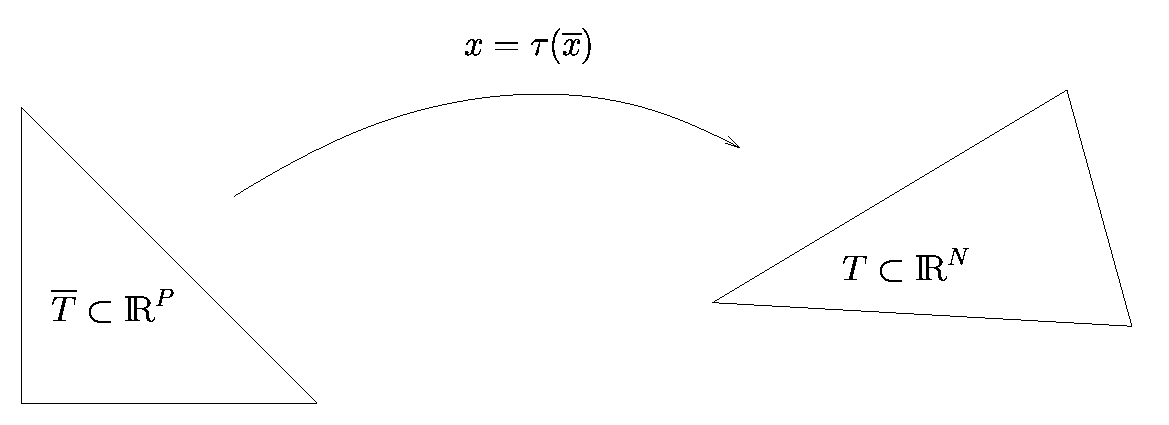
\includegraphics[width=10cm,angle=0]{getfemelem_trans.eps}
  \end{center}
  \caption{ \it Geometric transformation }
  \label{fig:transgeo}
\end{figure}

A geometric transformation is a polynomial application
$$ \tau : \overline{T} \subset \Reel^P \longrightarrow T \subset\Reel^N, $$
which maps the reference element $\overline{T}$ to the real element $T$.
The geometric nodes are denoted
$$ g^i, \ \ i = 0 .. n_g - 1. $$
The geometric transformation is described thanks to a $n_g$ components polynomial vector
$$ {\cal N}(\overline{x}), $$
such that
$$ \tau(\overline{x}) = \sum_{i = 0}^{n_g - 1} {\cal N}_i(\overline{x}) g^i.$$
Denoting
$$ G = (g^0; g^1; ...; g^{n_g - 1}), $$
the $N \times n_g$ matrix containing of all the geometric nodes, one has
$$ \fbox{$\hspace{1em}\tau(\overline{x}) = G {\cal N}(\overline{x}).\hspace{1em}$} $$
The derivative of $\tau$ is then
$$ \fbox{$\hspace{1em} K(\overline{x}) := \nabla \tau(\overline{x}) = G \nabla {\cal N}(\overline{x}),\hspace{1em}$} $$
where $K(\overline{x}) = \nabla \tau(\overline{x})$ is a $N \times P$ matrix and $\nabla {\cal N}(\overline{x})$ a $n_g \times P$ matrix.
The (transposed) pseudo-inverse of $\nabla\tau(\overline{x})$ is a $N\times P$ matrix denoted $B(\overline{x})$:
$$ \fbox{$\hspace{1em} B(\overline{x}) := K(\overline{x})(K(\overline{x})^T K(\overline{x}))^{-1},\hspace{1em}$} $$
Of course, when $P=N$, one has $B(\overline{x})=K(\overline{x})^{-T}$.

Pointer on a descriptor of a geometric transformation can be obtained by the following function defined in the file {\tt bgeot\_geometric\_trans.h}:\\[0.5cm]
{\tt bgeot::pgeometric\_trans pgt = bgeot::geometric\_trans\_descriptor("name of trans"); }\\[0.5cm]
where {\tt "name of trans"} should be chosen among the following list.
\begin{center} \begin{tabular}{|m{0.3\linewidth}|m{0.65\linewidth}|} \hline
{\tt "GT\_PK(n,k)"} & Description of the simplex transformation of dimension {\tt n} and degree {\tt k} (Most of the time, the degree 1 is used).\\ \hline
{\tt "GT\_QK(n,k)"} & Description of the parallelepiped transformation of dimension {\tt n} and degree {\tt k}.\\ \hline
{\tt "GT\_PRISM(n,k)"} & Description of the prism transformation of dimension {\tt n} and degree {\tt k}. \\ \hline
{\tt "GT\_PRODUCT(a,b)"} & Description of the direct product of the two transformations {\tt a} and {\tt b}.\\ \hline
{\tt "GT\_LINEAR\_PRODUCT(a,b)"} & Description of the direct product of the two transformations {\tt a} and {\tt b} keeping a linear transformation (this is a restriction of he previous function). This allows, for instance, to use exact integrations on regular meshes with parallelograms.\\ \hline
\end{tabular} \end{center}

\subsection{Inversion of geometric transformations}
The file {\tt bgeot\_geotrans\_inv.h} provides tools to invert geometric transformations. Those can be used for example to find out, among a list of points, which ones are inside a given convex.\\[0.5cm]
{\tt bgeot::geotrans\_inv gti; }\\[0.5cm]
To add the list off points to the object use\\[0.5cm]
{\tt gti.add\_point(pt);  }\\[0.5cm]
The points to be localized are selected via a ``kd-tree'', which is basically a generalisation of binary trees to more than one dimension.

The following function \\[0.5cm]
{\tt size\_type nb = gti.points\_in\_convex(cv, pgt, ptab, itab); }\\[0.5cm]
selects the points in the convex given by {\tt cv} and the geometric transformation {\tt pgt}.  To find which points are in a given element, the following algorithm is applied : \\
- compute a englobing box of the element, assuming that this element,
even if the geometric transfrmation in non-linear is in the englobing
box of its nodes times a factor 1.2, \\
- List all the points in this englobing box (via the kd-tree), \\
- For each points, invert the geometric transformation (computation
of a pseudo inverse in the linear case, and use of a Newton method in
the non-linear case. \\ \\
The inversion (i.e. finding $\overline{x}$ such that $\overline{x}=\tau{x}$, where $x$ is know in the real element) can be described as follows : \\ \\
\subsubsection*{Linear case}
If $\tau$ is linear (affin in fact), then \\
$$x = \tau(\overline{x}) = \nabla \tau(0) \overline{x} + x_0. = K(0)\overline{x} + x_0$$ \\
Hence
$$\fbox{$\overline{x} = B(0)^T(x - x_0)$}$$
if $N > P$, the residu \\
$$x - x_0 -  K(0) \overline{x}, $$
indicates wether or not the point $x$ in on the "surface" of the convex. \\ 
\\ \subsubsection*{Non-linear case}
A Newton method is applied., writing
$$x = \tau(\overline{x}+\overline{h}) = \tau(\overline{x})
+ \nabla \tau(\overline{x})\overline{h} + o(\|\overline{h}\|^2). $$
It gives the iterative scheme
$$\fbox{$ \overline{x}_{n+1} = \overline{x}_{n}
+ B^T(\overline{x}_{n})(x - \tau(\overline{x}_{n})).$} $$
The residu is
$$ x - \tau(\overline{x}_{n}).$$

\section{Finite element methods description}

A finite element method is defined on a reference element $\overline{T} \subset \Reel^P$ by a set of $n_d$ nodes $a^i$ and corresponding base functions 
$$ \overline{\varphi}^i : \overline{T} \subset \Reel^P \longrightarrow \Reel^Q, $$
Denoting
$$ \tilde{\varphi}^i(x) = \overline{\varphi}^i(\overline{x}) = \overline{\varphi}^i(\tau^{-1}(x)), $$
a linear transformation is allowed for the real base function
$$ \varphi^i(x) = \sum_{j = 0}^{n_d - 1} \tilde{M}_{ij} \tilde{\varphi}^j(x), $$
where $\tilde{M}$ is a $n_d \times n_d$ matrix possibly depending on the geometric transformation (i.e. on the real element). For basic elements as Lagrange elements this matrix is the identity matrix (it is simply ignored). In this case, we will say that the element is $\tau$-equivalent. This approach allows to define hermite elements (Argyris for instance) in a generic way, even with non linear transformations (i.e. mainly for curved boundaries).
We denote
$$ [\overline{\varphi}(\overline{x})] = \vecfour{\overline{\varphi}^0(\overline{x})}{\overline{\varphi}^1(\overline{x})}{...}{\overline{\varphi}^{n_d-1}(\overline{x})}, $$
the $n_d \times Q$ matrix, such that when a function is defined by
$$ f(x) = \sum_{i = 0}^{n_d - 1} \alpha_i \varphi^i(x), $$
one has
$$ \fbox{$\hspace{1em} f(\tau(\overline{x})) = \alpha^T \tilde{M} [\overline{\varphi}(\overline{x})],\hspace{1em}$} $$
where $\alpha$ is the vector of components $\alpha_i$.

A certain number of description of classical finite element method are defined in the file {\tt getfem\_fem.h}. More classical ones are the following (see \cite{FEM_LIST} for an exhaustive list):

\begin{center} \begin{tabular}{|m{0.55\linewidth}|m{0.4\linewidth}|} \hline
{\tt getfem::ppolyfem getfem::PK\_fem(n, k)} & Classical $P_K$ methods on simplexes of dimension  {\tt n} with degree {\tt k} polynomials.\\ \hline
{\tt getfem::ppolyfem getfem::QK\_fem(n, k)} & Classical $Q_K$ methods on parallelepiped of dimension {\tt n}. Tensorial product of degree {\tt k} $P_K$ method on the segment. \\ \hline
{\tt getfem::ppolyfem getfem::PK\_prism\_fem(n, k)} & Classical methods on prism of dimension {\tt n}. Tensorial product of two degree {\tt k} $P_K$ method. \\ \hline
{\tt getfem::ppolyfem getfem::product\_fem( ppolyfem\;a, ppolyfem b)} & Tensorial product of the two polynomial finite element method {\tt a} and {\tt b}. \\ \hline
{\tt getfem::ppolyfem $\;$ getfem::P1\_nonconforming\_fem()} & Non conforming $P_1$ method on triangles. \\ \hline
\end{tabular} \end{center}

One can obtain a particular descriptor thanks to the function\\[0.5cm]
{\tt getfem::pfem pfe = getfem::fem\_descriptor("name of method"); }\\[0.5cm]
One can see in the file {\tt getfem\_fem.C} how to define a new finite element method. Basically, the only thing to do is to give the base functions on the reference element and the corresponding nodes.

\section{Integration methods}

The integrations methods are of two kinds. The file {\tt getfem\_integration.h} defines approximated and exact integrations methods. The exact integration can only be used if all the elements are polynomial and if the geometric transformation is linear.

The following exact methods are defined

\begin{center} \begin{tabular}{|m{0.55\linewidth}|m{0.4\linewidth}|} \hline
{\tt "IM\_EXACT\_SIMPLEX(n)"} & Description of the exact integration of polynomials on the simplex of reference of dimension {\tt n}. \\ \hline
\end{tabular}  
\begin{tabular}{|m{0.55\linewidth}|m{0.4\linewidth}|} \hline
{\tt "IM\_PRODUCT(a, b)"} & Description of the exact integration on the convex which is the direct product of the convex in {\tt a} and in {\tt b}.\\ \hline
\end{tabular}  
\begin{tabular}{|m{0.55\linewidth}|m{0.4\linewidth}|} \hline
{\tt "IM\_EXACT\_PARALLELEPIPED(n)"} & Description of the exact integration of polynomials on the parallelepiped of reference of dimension {\tt n}\\ \hline
\end{tabular}  
\begin{tabular}{|m{0.55\linewidth}|m{0.4\linewidth}|} \hline
{\tt "IM\_EXACT\_PRISM(n)"} & Description of the exact integration of polynomials on the prism of reference of dimension {\tt n}\\ \hline
\end{tabular} \end{center}


Even though a description of exact integration method exists on parallelepipeds or prisms, most of the time the geometric transformations on such elements are not linear and the exact integration cannot be used.

Some examples of approximated methods (see \cite{FEM_LIST} for an exhaustive list):
\begin{center} \begin{tabular}{|m{0.55\linewidth}|m{0.4\linewidth}|} \hline
{\tt "IM\_GAUSS1D(k)" } & Description of the Gauss integration on a segment of order {\tt k}. \\ \hline
\end{tabular}  
\begin{tabular}{|m{0.55\linewidth}|m{0.4\linewidth}|} \hline
{\tt "IM\_NC(n,k)"} & Description of the integration on a simplex of reference of dimension {\tt n} for polynomials of degree {\tt k} with the Newton Cotes method (based on Lagrange interpolation).\\ \hline
\end{tabular}  
\begin{tabular}{|m{0.55\linewidth}|m{0.4\linewidth}|} \hline
{\tt "IM\_PRODUCT(a,b)"} & Build a method doing the direct product of methods {\tt a} and {\tt b}. \\ \hline
\end{tabular}  
\begin{tabular}{|m{0.55\linewidth}|m{0.4\linewidth}|} \hline
{\tt "IM\_TRIANGLE(2)"} & Integration on a triangle of order 2 with 3 points. \\ \hline
\end{tabular}
\begin{tabular}{|m{0.55\linewidth}|m{0.4\linewidth}|} \hline
{\tt "IM\_TRIANGLE(7)"} & Integration on a triangle of order 7 with 13 points. \\ \hline
\end{tabular} 
\begin{tabular}{|m{0.55\linewidth}|m{0.4\linewidth}|} \hline
{\tt "IM\_QUAD(2)"} & Integration on quadrilaterals of order 2 with 3 points. \\ \hline
\end{tabular}
\begin{tabular}{|m{0.55\linewidth}|m{0.4\linewidth}|} \hline
{\tt "IM\_TETRAHEDRON(5)"} & Integration on a tetrahedron of order 5 with 15 points. \\ \hline
\end{tabular} \end{center}


One can obtain a particular descriptor thanks to the function\\[0.5cm]
{\tt getfem::pintegration\_method pfe = getfem::int\_method\_descriptor("name of method"); }\\[0.5cm]


\section{Mathematical description of basic calculus}

\subsection{Volume integral}
One has
$$ \int_T f(x) dx = \int_{\overline{T}} \overline{f}(\overline{x}) |vol\left(\Frac{\partial \tau(\overline{x})}{\partial \overline{x}_0} ;\Frac{\partial \tau(\overline{x})}{\partial \overline{x}_1}; ...; \Frac{\partial \tau(\overline{x})}{\partial \overline{x}_{P-1} }\right)| d\overline{x}, $$
with
$$ \fbox{$\hspace{1em} J_{\tau}(\overline{x}) := |vol\left(\Frac{\partial \tau(\overline{x})}{\partial \overline{x}_0} ;\Frac{\partial \tau(\overline{x})}{\partial \overline{x}_1}; ...; \Frac{\partial \tau(\overline{x})}{\partial \overline{x}_{P-1} }\right)| = (\mbox{det}(K(\overline{x})^T K(\overline{x})))^{1/2},\hspace{1em}$} $$
one finally has
$$ \fbox{$\hspace{1em} \ds \int_T f(x) dx = \int_{\overline{T}} \overline{f}(\overline{x})  J_{\tau}(\overline{x})d\overline{x}.\hspace{1em}$} $$
When $P = N$, of course $J_{\tau}(\overline{x}) = |\mbox{det}(K(\overline{x}))|$.

\subsection{Surface integral}
With $\Gamma$ a part of the boundary of $T$ a real element and $\overline{\Gamma}$ the corresponding boundary on the reference element $\overline{T}$ and, one has
$$ \fbox{$\hspace{1em} \ds \int_{\Gamma} f(x) d\sigma = \int_{\overline{\Gamma}} \overline{f}(\overline{x}) \|B(\overline{x})\overline{\mathbf n}\| J_{\tau}(\overline{x}) d\overline{\sigma},\hspace{1em}$} $$
where ${\mathbf n}$ is the unit normal to $\overline{T}$ on $\overline{\Gamma}$. On a same manner
$$ \fbox{$\hspace{1em} \ds \int_{\Gamma} F(x).{\mathbf n} d\sigma = \int_{\overline{\Gamma}} \overline{F}(\overline{x}).(B(\overline{x})\overline{\mathbf n}) J_{\tau}(\overline{x}) d\overline{\sigma}.\hspace{1em}$} $$

\subsection{Derivative computation}
One has
$$ \nabla f(x) = B(\overline{x}) \overline{\nabla}\,\overline{f}(\overline{x}), $$
\subsection{Second derivative computation}
Denoting 
$$ \nabla^2 f = ({\Frac{\partial^2 f}{\partial x_i \partial x_j}})_{ij}, $$
the $N \times N$ matrix and
$$ \overline{X}(\overline{x}) = \sum_{k = 0}^{N-1} \overline{\nabla}^2 \tau_k(\overline{x}) \Frac{\partial f}{\partial x_k}(x) = \sum_{k = 0}^{N-1} \sum_{i = 0}^{P-1} \overline{\nabla}^2 \tau_k(\overline{x}) B_{ki} \Frac{\partial \overline{f}}{\partial \overline{x}_i}(\overline{x}), $$
the $P \times P$ matrix, then
$$ \overline{\nabla}^2 \overline{f}(\overline{x}) = \overline{X}(\overline{x}) + K(\overline{x})^T \nabla^2 f(x) K(\overline{x}), $$
and thus
$$ \nabla^2 f(x) = B(\overline{x}) (\overline{\nabla}^2 \overline{f}(\overline{x}) - \overline{X}(\overline{x})) B(\overline{x})^T. $$

In order to have uniform methods for the computation of elementary matrices, the Hessian is computed as a vector:
$$  H f = \vecseven{\Frac{\partial^2 f}{\partial x^2_0}}{}{\Frac{\partial^2 f}{\partial x_1 \partial x_0}}{}{\Frac{\partial^2 f}{\partial x_2 \partial x_0}}{...}{\Frac{\partial^2 f}{\partial x^2_{N-1}}},\ \ \ \ \ 
    \overline{H}\,\overline{f} = \vecseven{\Frac{\partial^2 \overline{f}}{\partial \overline{x}^2_0}}{}{\Frac{\partial^2 \overline{f}}{\partial \overline{x}_1 \partial \overline{x}_0}}{}{\Frac{\partial^2 \overline{f}}{\partial \overline{x}_2 \partial \overline{x}_0}}{...}{\Frac{\partial^2 \overline{f}}{\partial \overline{x}^2_{P-1}}}, $$
Then, with $B_2$ the $P^2 \times P$ matrix defined as
$$ \fbox{ $(B_2(\overline{x}))_{ij} = \sum_{k = 0}^{N-1} \Frac{\partial^2 \tau_k(\overline{x})}{\partial \overline{x}_{i / P} \partial \overline{x}_{i \mbox{ mod } P} } B_{kj}(\overline{x}),$ } $$
and $B_3$ the $N^2 \times P^2$ matrix defined as
$$ \fbox{ $(B_3(\overline{x}))_{ij} = B_{i / N, j / P}(\overline{x}) B_{i \mbox{ mod } N, j \mbox{ mod } P}(\overline{x}), $ } $$
then
$$ \fbox{ $H f(x) = B_3(\overline{x}) \left(\overline{H}\,\overline{f}(\overline{x}) - B_2(\overline{x})\overline{\nabla}\,\overline{f}(\overline{x})\right), $ } $$

\subsection{Example of elementary matrix} \label{elmminst}

Assume one needs to compute the elementary ``matrix'':
$$ t(i_0, i_1, ..., i_7) = \int_{T} \varphi_{i_1}^{i_0}\; \partial_{i_4} \varphi_{i_3}^{i_2}\; \partial^2_{i_7 / P, i_7 \mbox{ mod } P} \varphi_{i_6}^{i_5} dx, $$ 
The computations to be made on the reference elements are
$$ \overline{t}_0(i_0, i_1, ..., i_7) = \int_{\overline{T}} \overline{\varphi}_{i_1}^{i_0}\; \partial_{i_4} \overline{\varphi}_{i_3}^{i_2}\; \partial^2_{i_7 / P, i_7 \mbox{ mod } P} \overline{\varphi}_{i_6}^{i_5}  J(\overline{x}) d\overline{x}, $$
and
$$ \overline{t}_1(i_0, i_1, ..., i_7) = \int_{\overline{T}} \overline{\varphi}_{i_1}^{i_0}\; \partial_{i_4} \overline{\varphi}_{i_3}^{i_2}\; \partial_{i_7} \overline{\varphi}_{i_6}^{i_5}  J(\overline{x}) d\overline{x}, $$
Those two tensor can be computed once on the whole reference element if the geometric transformation is linear (because $J(\overline{x})$ is constant). If the geometric transformation is non-linear, what has to be stored is the value on each integration point. To compute the integral on the real element a certain number of reductions have to be made:
\begin{itemize}
   \item Concerning the first term ($\varphi_{i_1}^{i_0}$) nothing.
   \item Concerning the second term ($\partial_{i_4} \varphi_{i_3}^{i_2}$) a reduction with respect to $i_4$ with the matrix $B$.
   \item Concerning the third term ($\partial^2_{i_7 / P, i_7 \mbox{ mod } P} \varphi_{i_6}^{i_5}$) a reduction of $\overline{t}_0$ with respect to $i_7$ with the matrix $B_3$ and a reduction of $\overline{t}_1$ with respect also to $i_7$ with the matrix $B_3B_2$
\end{itemize}
The reductions are to be made on each integration point if the geometric transformation is non-linear. Once those reductions are done, an addition of all the tensor resulting of those reductions is made (with a factor equal to the load of each integration point if the geometric transformation is non-linear).

If the finite element is non-$\tau$-equivalent, a supplementary reduction of the resulting tensor with the matrix $\tilde{M}$ has to be made.

\section{Elementary matrices description}

Before to compute a particular elementary matrix one has to obtain a descriptor  of this elementary matrix. The basic descriptor are defined in the file {\tt getfem\_mat\_elem\_type.h}. 

\begin{center} \begin{tabular}{|m{0.55\linewidth}|m{0.4\linewidth}|} \hline
{\tt getfem::pmat\_elem\_type getfem::mat\_elem\_base(getfem::pfem pfi) } & Elementary matrix which computes the integral of each base functions (in fact each component of each base function)\\ \hline
{\tt getfem::pmat\_elem\_type getfem::mat\_elem\_grad(getfem::pfem pfi) } & Elementary matrix which computes the integral of the gradient of each base functions\\ \hline
{\tt getfem::pmat\_elem\_type getfem::mat\_elem\_hess(getfem::pfem pfi) } & Elementary matrix which computes the integral of the Hessian of each base functions\\ \hline
{\tt getfem::pmat\_elem\_type getfem::mat\_elem\_product(pmat\_elem\_type a, pmat\_elem\_type b) } & Elementary matrix which computes the integral of the product of what is computed in {\tt a} and {\tt b}. \\ \hline
\end{tabular} \end{center}

For instance if one wants the description of the elementary matrix given in Section \ref{elmminst} one can obtain it as
{\tt getfem::pmat\_elem\_type pet = getfem::mat\_elem\_product(\\
    $\mbox{}$\hspace{10em} getfem::mat\_elem\_product(getfem::mat\_elem\_base(pfi), \\
     $\mbox{}$\hspace{22.5em}      getfem::mat\_elem\_grad(pfi)),\\
     $\mbox{}$\hspace{22.5em}      getfem::mat\_elem\_hess(pfi));
}


\section{Elementary matrices computation, order of indices}

The file {\tt getfem\_mat\_elem.h} provides objects which are capable to compute elementary matrices.  There are three parameters to build those objects : a description of the elementary matrix (which contains information on the finite element methods), a description of the integration method and the geometric transformation.

\begin{center} \begin{tabular}{|m{0.55\linewidth}|m{0.4\linewidth}|} \hline
{\tt getfem::pmat\_elem\_computation mat\_elem(pmat\_elem\_type pm, pintegration\_method pi, pgeometric\_trans\;pg)} & Gives a pointer to the object which is able to compute the elementary matrix. \\ \hline
\end{tabular} \end{center}

This object has two generic methods which can be called to actually compute the elementary matrices :

\begin{center} \begin{tabular}{|m{0.55\linewidth}|m{0.4\linewidth}|} \hline
{\tt pmec->gen\_compute(base\_tensor \&t, const CONT \&a)} & Compute the elementary matrix in the tensor {\tt t} (and adjust sizes if necessary). The variable {\tt a} is any container containing the list of the vertices of the real element\\ \hline
{\tt pmec->gen\_compute\_on\_face(base\_tensor \&t, const CONT \&a, f)} & Compute the elementary matrix on the face {\tt f} of the element in the tensor {\tt t} (and adjust sizes if necessary). The variable {\tt a} is any container containing the list of the vertices of the real element\\ \hline
\end{tabular} \end{center}

\underline{Order of indices in the tensor {\tt t} follows the example in section \ref{elmminst}}

\section{Example of use (OBSOLETE)}
In the file {\tt getfem\_assembling.h}, one can see some examples of use of the elementary matrices computation. This file contains a certain number of assembling functions for classical problems systems (linear elasticity, Laplacian Stokes problem ...).

\subsection{Elementary matrix for the Laplacian with $P_1$ element}

To assemble the rigidity matrix for the Laplacian, one needs the integrals
$$ \int_T \partial_j \phi^i(x) \partial_l \phi^k(x) dx, $$
where $\phi^i$ are the base functions on the real element $T$ (even though for this problem all the components will not be used). Those elementary computations can be obtained with the following code for the $P_1$ finite element method:

\begin{alltt}
#include<getfem_mat_elem.h>

int main(void) \{
  int N = 3;                // dimension
  char method\_name[100];
  char gt\_name[100];
  getfem::base_tensor t;    // tensor for the computation of elementary matrix

  sprintf(method\_name, "FEM\_PK(\%d, \%d)", N, 1);
  getfem::pfem pf = getfem::fem\_descriptor(method\_name); // P_1 method, dimension N

  getfem::pmat_elem_type pet = // Type of elementary matrix
     getfem::mat_elem_product(getfem::mat_elem_grad(pf),
                              getfem::mat_elem_grad(pf));

  sprintf(method\_name, "IM\_EXAXT\_SIMPLEX(\%d)");
  sprintf(gt\_name, "GT\_PK(\%d, \%d)", N, 1);
  getfem::pmat_elem_computation pmec = // Object which computes elementary matrices.
     getfem::mat_elem(pet, getfem::int\_method\_descriptor(method\_name),
                           bgeot::geometric\_trans\_descriptor(gt\_name));

  std::vector<base_node> A(N+1);  // Build a list of vertices.
  base_node pt;  // Of course, usually, the real vertices come from the mesh
  std::fill(pt.begin(), pt.end(), 0.0);
  std::fill(A.begin(), A.end(), pt);
  for (int i = 0; i < N; ++i)
    A[i+1][i] = 1.0;

  // Computation of the elementary matrix on the real element
  pmec->gen_compute(t, A);

  cout << t; // ... and do what you want with t  

  // Computation of the elementary matrix on the face 0 of the real element
  pmec->gen_compute_on_face(t, A, 0); 

  cout << t; // ... and do what you want with t  

\}

\end{alltt}

\subsection{Elementary matrix for a mixed $P_1, P_2$ element}

To assemble certain mixed problems (such as for the Stokes problem for instance) one may need the following integrals:
$$ \int_T \phi^i(x) \partial_k \psi^j(x) dx, $$
where $\phi^i$ are the base functions of the $P_1$ finite element method, and $\psi^j$ are the base functions of the $P_2$ finite element method. To obtain this, the following lines have to replace the corresponding lines in the code of the latter section.

\begin{alltt}

  sprintf(method\_name, "FEM\_PK(\%d, \%d)", N, 1);
  getfem::pfem pf1 = getfem::fem\_descriptor(method\_name); // P_1 method, dimension N
  sprintf(method\_name, "FEM\_PK(\%d, \%d)", N, 2);
  getfem::pfem pf2 = getfem::fem\_descriptor(method\_name); // P_2 method, dimension N  

  getfem::pmat_elem_type pet = // Type of elementary matrix
     getfem::mat_elem_product(getfem::mat_elem_base(pf1),
                              getfem::mat_elem_grad(pf2));
                              
\end{alltt}


\begin{thebibliography}{99}
% \bibliographystyle{apalike}
% \bibliographystyle{plain}
% \bibliography{all}
\bibitem{dh-to1984} 
  G. {\sc Dhatt, and  G. Touzot}
  {\it The Finite Element Method Displayed}, 
 J. Wiley \& Sons,  New York, 1984.

\bibitem{FEM_LIST}
  Y. {\sc Renard},
  {\it Description of Finite Element and Integration Methods in {\sc Getfem++}}, 2002.


\end{thebibliography}
\end{document}
